\section{Hypotheses}

RJCB expects that the inference error is lowest when the true
tree is generated under MBD parameter settings without multiple-births, i.e
$nu = 0 \vee q = 0$. For such parameters settings, the
true is in practice generated by a BD model, which
matches the tree prior used in inference. Without a mismatch between
true tree prior and assumed tree prior, this source of errors will be absent,
where the other two sources of errors (stochasticity in the
simulation of the alignment and the MCMC algorithm) 
will remain the same.

RJCB expects that, on average, the inference error is highest for
parameter settings with a higher percentage of multiple-births,
i.e. $nu > 0 \wedge q > 0$, as for these settings, 
the mismatch between the the speciation model that
generated the true tree (which is profoundly-MB MBD) is biggest with
the tree prior assumed to be generative (which is BD).

RJCB expects that the inference error is higher for true trees
with a higher percentage of species generated in an MB event,
regardless of the MBD parameters.
These multiple-born species are one of the three (and the most 
interesting) sources of error, as a BD model -as a feature- will never
infer a co-occuring speciation event.

RJCB expects that an increased extinction rate
has a neutral effect on the error made, 
for runs with an equal percentage of MBness,
because extinction affects all species equally. 

RJCB expects that an increased number of taxa
has a negative effect on the variance of the errors made, as there
is more information available to base inference on.

RJCB expects that an increased extinction rate
increases the variance of the errors made,
due to the decrease of the number of taxa, reducing the amount of information
to base inference on.

RJCB expects that the nLTT statistic between a true and twin
tree at the start of the pipeline,
will correlate strongly with the difference
between the higest posterior density of the 
errors of the true and twin tree 
generated at the end of the pipeline. 
This hypothesis
stems from the idea of assuming a setup without noise; that is, with
a DNA alignment of infinite length. From such a DNA alignment 
with infinite information, the MCMC
is able to infer the close-to-correct phylogeny.
\richel{if this is true, we can use this shortcut (instead of running
multiple pirouette replicates) to draw stronger conclusions}

\begin{figure}[!htbp]
  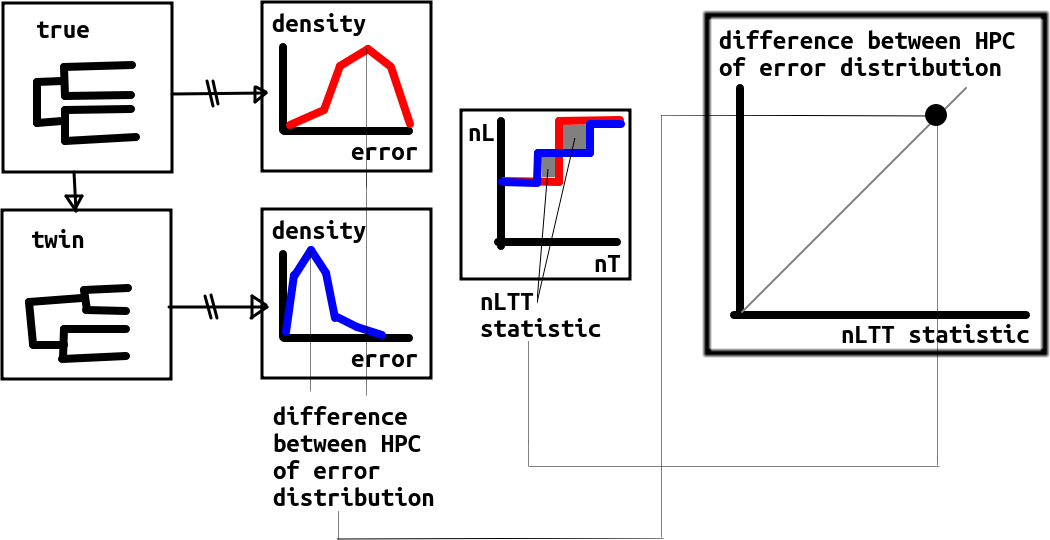
\includegraphics[width=\textwidth]{20191126_nltt_as_proxy.png}
  \caption{
    The nLTT statistic between true and twin tree correlates strongly
    with the difference between (the highest posterior density
    of) the errors of the true and twin tree.
  }
  \label{fig:nltt_as_proxy}
\end{figure}

